% -----
% COMP2550 proposal
% CHRISTOPHER CLAOUE-LONG
% -----
% -
% - DOCUMENT GEOMETRY SETUP
\documentclass[12pt,a4paper]{article}
\usepackage[margin=20mm]{geometry}
\usepackage{wrapfig}
\usepackage{lastpage} % to display the page number down the bottom
\makeatletter \renewcommand{\@oddfoot}{\hfil Page \thepage\ of \pageref{LastPage} \hfil} \makeatother % Page X of Y down the bottom
% -
% - FONT
\usepackage{amsmath,amsthm,amssymb,graphicx,epstopdf,datetime,multicol,verbatim,ulem,alltt,multirow}
\DeclareGraphicsRule{.tif}{png}{.png}{`convert #1 `dirname #1`/`basename #1 .tif`.png}
\usepackage[sc]{mathpazo} % Palatino maths fonts - acceptable fonts for typesetting, also sets these fonts for use in math mode
\linespread{1.05}
\usepackage[T1]{fontenc}
\usepackage[bitstream-charter]{mathdesign}
% -
% - MISC. PACKAGES
\usepackage[usenames,dvipsnames,svgnames,table]{xcolor}
\usepackage{hyperref}
\hypersetup{
colorlinks,
citecolor=black,		% - Citation colour
filecolor=black,		% - File colour
linkcolor=black,		% - Link colour
urlcolor=black		% - URL colour
}\urlstyle{same}
% -
% -
% - MISC. SYMBOLS AND COMMANDS
\newcommand{\HUGE}[1]{\textbf{\Huge #1}}
\newcommand{\ITALIC}[1]{\textit{#1}}
\newcommand{\BOLDL}[1]{\textbf{\large #1}}
\newcommand{\BOLD}{\textbf}
\newcommand{\Hrule}{\textcolor{blue}{\rule{\linewidth}{0.5mm}}} 

% Defines a new command for the horizontal lines, change thickness here
\newcommand{\htab}{\hspace*{0.63cm}}
\newcommand{\SUPER}{\textsuperscript}
\newenvironment{Figure}
  {\par\medskip\noindent\minipage{\linewidth}}
  {\endminipage\par\medskip}
\newcommand{\TIMELINE}[3]{#1\\\BOLD{#2} #3}
\newcommand{\TIMELINESPACE}{\\[0.3cm]}
% -
% -----
% BEGIN DOCUMENT
% -----
\begin{document}
% -----
% - Title
{\center{\Hrule\vspace{0.2em}
	%
	\HUGE{COMP2550/COMP3130 ANU\\Main Project Proposal}\\
	\BOLDL{
		Christopher Claou\'e-Long
		(\href{mailto:u5183532@anu.edu.au}
		{\ITALIC{\underline{\smash{u5183532@anu.edu.au}}}})\\
		Jimmy Lin 
		(\href{mailto:u5223173@anu.edu.au}
		{\ITALIC{\underline{\smash{u5223173@anu.edu.au}}}})\\
	}
\Hrule}}
%
% -
\begin{multicols}{2}
\section{Introduction}
\htab A long-standing problem in the field of computer vision is how to calculate the saliency of objects in images, that is the prominence of them compared to the background.  This property is important for image recognition via computer vision because it enables automatic image cropping and adaptive image display on small screens as well as enhanced image and video compression.\\
% -
% introduce related work 
\htab Today, there are a few existing works that achieve a high accuracy in detecting salient objects. The most recognised approach in the last decade is Itti's algorithm from 1998 (see ref.3). It calculates a feature map and then converts it to a rectangle via a winner-take-all algorithm. However, the precision of the detection from this and other algorithms is as yet unsatisfying, even though Itti's algorithm in particular has good object recall. Another approach is to use fuzzy-growing (see ref.4), which directly labels saliency in a less costly way. However, it trades accuracy for its speed, shown in the following comparison.
% -
% image outlining salient object detection
\begin{Figure}
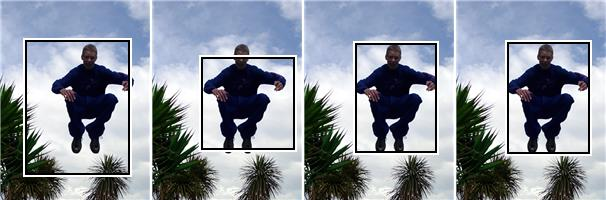
\includegraphics[width=3.2in,height=1in]{./pictures/0_imCanvs_Compare.jpg} \\
{\htab \tiny (a) FG(Ma,2003) (b) SM(Itti,1998) (c) CRFM(Liu,2007) (d) Ground truth}
\end{Figure}
% -
% framework
The research we will be referring to to in this experimental project is that of Liu, Tie et al. in 2011 (see ref.2), which is based on a conditional random field (CRF) model.  This allows a large amount of near-perfect saliency detection compared with the ground truth data. To accomplish this, it extracts features on the local, regional and global levels, where it calculates multiscale contrast, a centre-surround histogram and a spatial color distribution respectively. After normalization and combination via an energy function, a master map, better known as a salient map, is computed to represent the saliency of each pixel in the image. A few key locations on the saliency map are finally identified through a winner-take-all or inhibition-of-return algorithm, as well as  other non-linear operations that act on the probability of a salient object being present at the location.
% -
% implementation details
\section{Proposed Implementation}
% implementation outline and explanation of chice
\htab Our implementation will employ the  OpenCV library, leveraging on the ANU's open source DARWIN framework (see ref.1) to achieve a CRF-based saliency detection algorithm. The reason for selecting CRF-based saliency detection as our project focus is that this project would give us experience in the manipulation of graphical models in practice, especially in the mechanisms of learning and inference by CRFs. Additionally, a scene understanding algorithm with dozens of class labels is expensive and complex compared to exclusively labelling the salient region and its near neighbourhood within a tremendously large image, so employing a CRF-based algorithm will result in a large reduction in the time required to run.
\subsection{Conditional Random Fields}
\htab Conditional Random Fields can model the saliency distribution in an image, given some known features about the surrounding pixels.  They can be described by the equation
    $$ P(A|I) = \frac{1}{Z} \cdot\exp(-E(A|I)) $$
where $A$ is the binary mask (salient or non-salient), I is the known pixel intensity and $E(A|I)$ is the energy function, formulated to be a set of static salient features and one pairwise feature as follows:
    $$ E(A|I) = \sum_{x} \sum_{k=1}^{K} \lambda_{k} F_{k}(a_{x},I)  
        + \sum_{x,x'} S(a_{x},a_{x'},I)  $$
$\lambda_{k}$: weight of $k$th feature, $x,x'$: two adjacent pixels. 
%
\subsection{Feature Extraction Ideas}
\textbf{Multiscale Contrast}. This static feature extracts intensity, color, orientation, and texture at multiple scales to capture the contrast in the boundary between objects . \\
\textbf{Center-Surround Histogram}. This static feature can be computed using various low-level features via a center-surround operation.  \\[0.1cm]
\textbf{Spatial Color distribution}. This static feature penalizes the pixels with widely distributed color. \\[0.1cm]
\textbf{Pairwise Feature}. This feature exploits the spatial relationship between two adjacent pixels and can be viewed as capturing the spatial continuity of saliency -- that is, adjacent pixels that are prone to be assigned with different labels. 
\subsection{Possible Improvements}
\htab One possible breakthrough lies in enhancing the quality of extracted features for detecting saliency. From the referred approach (Tie, ref.2), the saliency of animal legs (i.e. horses, elk) are frequently missed even in the feature maps, perhaps because of the thin width of the legs. Another possible improvement in this area is to create an algorithm capable of real-time saliency detection for application in video streams.
\section{Project Timeline}
\TIMELINE{1\SUPER{st}  - 18\SUPER{th} April}{Project Proposal:}{Research current literature to find papers and inspire a project of interest, determine the topic of our second project and collect relevant datasets for training.}\TIMELINESPACE
%
\TIMELINE{19\SUPER{th} April - 28\SUPER{th} April}{Framework Construction:}{Gain familiarity with the packages and existing frameworks and implementations in Darwin and OpenCV, set up the interface to accept training data and the CRF model for saliency learning and inference.} \TIMELINESPACE
%
\TIMELINE{29\SUPER{th} April - 12\SUPER{th} May}{Implementation:}{Design and implement algorithms to calculate various features and output a rectangle/rectangles labeling the salient object(s).}\TIMELINESPACE
%
\TIMELINE{12\SUPER{th} May- 19\SUPER{th} May}{Testing and Improvements:}{Test the framework, review or research possible improvements and implmenent.}\TIMELINESPACE
%
\TIMELINE{20\SUPER{th} May - 30\SUPER{th} May}{Project Review and Report:}{Write up report summarising our project and findings, prepare presentation.}
% References
\begin{thebibliography}{0} \footnotesize   \setlength{\itemsep}{-0.5pt}%
    \bibitem 1 Gould, Stephen. "DARWIN: A Framework for Machine Learning and Computer Vision Research and Development." \textit{Journal of Machine Learning Research 13 (2012): 3533-3537}. 
    \bibitem 2 Liu, Tie, et al. "Learning to detect a salient object." \textit{Pattern Analysis and Machine Intelligence, IEEE Transactions on 33.2 (2011): 353-367}. 
    \bibitem 3 Itti, Laurent, Christof Koch, and Ernst Niebur. "A model of saliency-based visual attention for rapid scene analysis."\textit{ Pattern Analysis and Machine Intelligence, IEEE Transactions on 20.11 (1998): 1254-1259}.
    \bibitem 4 Ma, Yu-Fei, and Hong-Jiang Zhang. "Contrast-based image attention analysis by using fuzzy growing."\textit{ Proceedings of the eleventh ACM international conference on Multimedia. ACM, 2003}. 
\end{thebibliography}
\end{multicols}
\vfill\Hrule
\end{document}
% -----
% END OF LINE
% -----
